\documentclass[12pt, a4paper, bibliography=totoc]{scrartcl}

% personal data
\date{\today}


% language
\usepackage{polyglossia}
\setmainlanguage{english}
\setotherlanguages{german}
\usepackage{microtype}
\usepackage{dcolumn}

\usepackage[style=numeric,
			natbib=true,
			backend=biber]{biblatex}		%Bibliographie
\usepackage[autostyle=true,
			 german=quotes]
			 {csquotes}					%Anführungszeichen
\usepackage{blindtext}


%math and theorems
\usepackage{amsmath}
\usepackage{amssymb}
\usepackage{amsopn}					%Matheoperatoren
\usepackage[amsmath,thmmarks,hyperref]{ntheorem}
\usepackage{mathtools}
\usepackage{mathdots}					%Punkte
\usepackage{dsfont}
\usepackage{upgreek}					%Griechische Buchstaben
\usepackage{bbm}						%Mengensymbol
\usepackage{physics}					%Physiksymbole
\usepackage{relsize}						%Größenangaben
\usepackage[separate-uncertainty,
			per-mode=symbol]
			{siunitx}					%Einheiten
%\usepackage{tikz}						%Zeichnen
\usepackage{upgreek}					%Griechische Buchstaben
\usepackage{enumitem}
\setlist{nolistsep}


%useful packages
%\usepackage{geometry}
\usepackage{xcolor}
\usepackage{graphicx}
\usepackage{float}
\usepackage{csquotes}
\usepackage{todonotes}
\usepackage{booktabs}
\usepackage{array}
\usepackage[labelfont=bf]{caption}
\usepackage{wrapfig}
\usepackage{enumitem}
%\usepackage{xr} % cross referencing
%\usepackage{titling}
%\usepackage{titlesec}
%\usepackage[Bjornstrup]
%			{fncychap}					%Kapitellayout


\setmainfont{Linux Libertine O}
\setsansfont{Linux Biolinum O}

\usepackage{scrhack}					%Verbesserung Pakete
\usepackage{xltxtra}						%fontec


\newcommand{\im}{\mathrm{i}}
\newcommand{\e}{\mathrm{e}}
\renewcommand{\pi}{\uppi}
\renewcommand{\epsilon}{\varepsilon}


\addbibresource{bibliography.bib}

%color settings
\definecolor{myred}{RGB}{196,19,47} 
\definecolor{myblue}{RGB}{0,139,139}


%appendix
\usepackage[toc,page]{appendix}

%killing indent
\setlength{\parindent}{0pt}
\usepackage{multicol}
\usepackage{siunitx}
\usepackage{hyperref}


\title{FP18 Atmospheric Trace Gases}
\author{Aaron Mielke \& Thomas Ackermann}
\date{\today}

\begin{document}

\begin{center}
	\makeatletter
	\thispagestyle{empty}
	\large{Fortgeschrittenen-Praktikum}	
	\hfill
    \large{Summer term 2019}
    \vspace{5mm}
	\rule{\textwidth}{0.2pt}
    \vfill
	\Huge\textbf{\@title} \\
	\vspace{10mm}
	\large{\@author} \\
	\normalfont
	\vfill	
	\makeatother
\end{center}

\normalsize
\newpage

\section*{Abstract}

This experiment was conducted in the scope of the advanced lab course in physics at the Heidelberg University. \\
The experiment was conducted in the week of the $8^\text{th}$ april, 2019.

\tableofcontents
\newpage

\begin{multicols}{2}

\section{Introduction}\label{sec:Intro}

\subsection{Zusammensetzung der Atmosphäre}\label{ssec:Comp_Atmo}

Die Atmosphäre der Erde besteht aus einer Mischung verschiedener Gase.
Tabelle \ref{fig:atm_comp} zeigt eine Liste der Hauptkomponenten.

\begin{center}

\begin{tabular*}{\linewidth}{c c c}
	\toprule
	Gas & Symbol & Rel. Anteil \\
	\midrule
	Stickstoff & \ch{N2} & $78.084 \%$ \\
    Sauerstoff & \ch{O2} & $20.942\%$ \\
    Argon & \ch{Ar} & 0.934 \% \\
    Kohlenstoffdioxid & \ch{CO2} & 358 \si{ppmv} \\
	\bottomrule
\end{tabular*}

    \captionof{table}{Gase in der Atmosphäre} %\cite{atm_components}
    \label{fig:atm_comp}
\end{center}


\subsection{Messgrößen}\label{ssec:Messgröße}

Die Konzentration eines Spurengases ist die Zahl der Moleküle pro Volumeneinheit.
Eine andere wichtige Größe ist das Mischverhältnis.
Sie gibt den relativen Anteil eines Spurengases im Vergleich zur Luftmenge an und wird mit \si{[ppm]} oder \si{[ppt]} angegeben. 

\subsection{DOAS}\label{ssec:DOAS}

\textit{Differential Optical Absorption Spectroscopy} (DOAS) wird verwendet um die Konzentration eines bestimmten Spurengases in der Atmosphäre zu bestimmen - was das Ziel dieses Experimentes ist.
Das Hauptprinzip ist das Folgende: 
    Man nimmt zwei Spektren auf, eines welches auf der Erde aufgenommen wurde (also mit Absorption des Sonnenlichtes durch die Atmosphäre) und eines bei dem die Atmosphäre nicht präsent ist (Von Satellit aus aufgenommen.)
Jedes Gas absorbiert bestimmte Wellenlängen des Sonnenlichts.

\begin{center}
    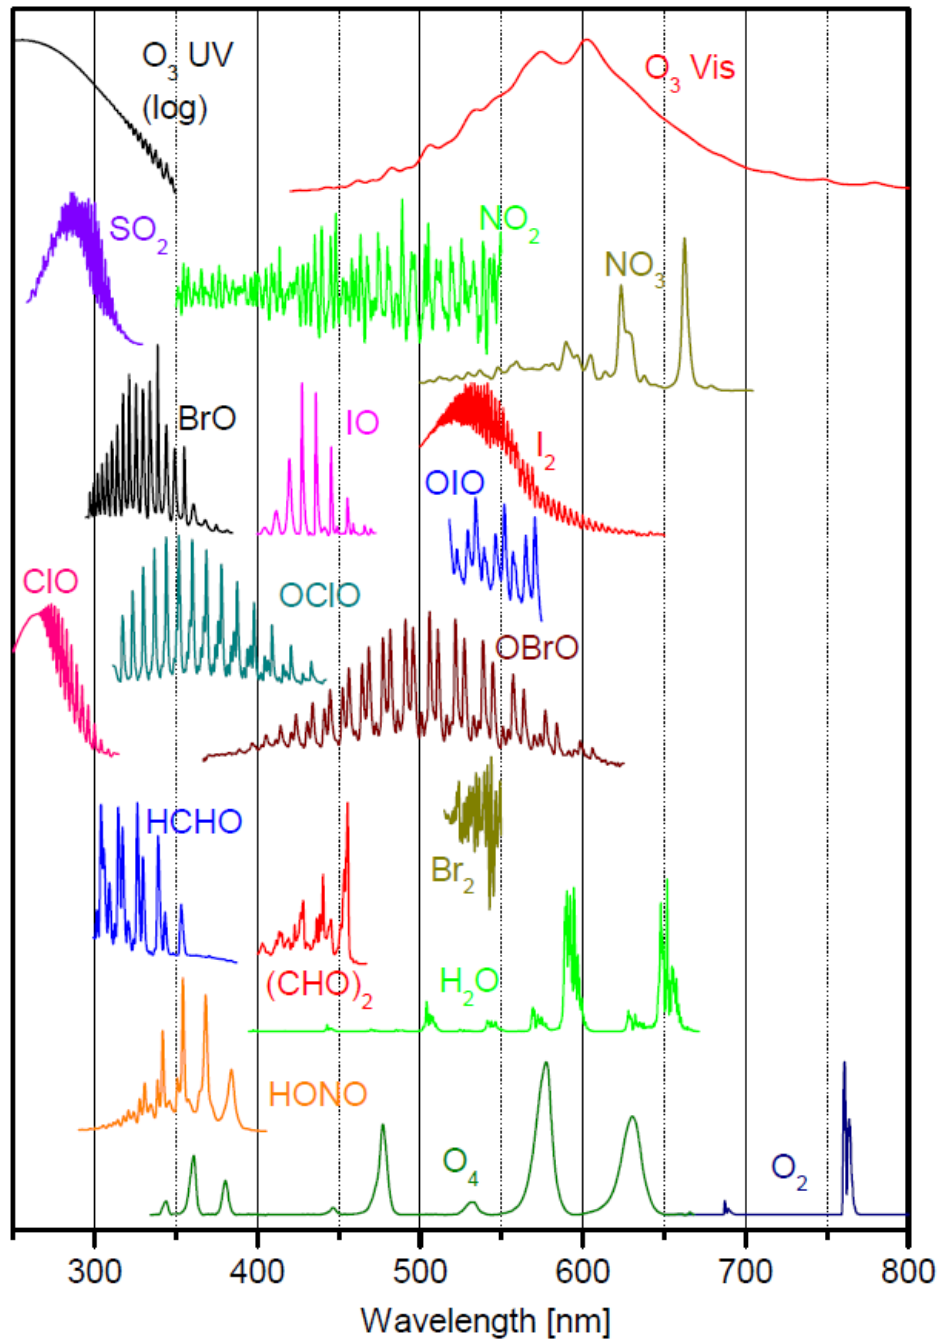
\includegraphics[width=0.7\linewidth]{fig/gas_spectra.png}
    \captionof{figure}{Charakteristische Linien verschiedener Gase}	
    \label{fig:gas_spectra}
\end{center}

Wenn nun zwei Spektren, wie beschrieben, aufgenommen werden 
können das charakteristische Verhalten der Gase daran erkannt werden dass die Intensitäten an manchen stellen kleiner sind.

Wenn man nun weiß welche Charakteristika zu welchen Gasen gehören kann die Dichte des Gases in der Atmosphäre bestimmt werden.
In diesem Versuchsaufbau steht allerdings kein Satellit zur Verfügung so dass sich die frage stellt wie man an ein Sonnenspektrum ohne Atmosphäre kommt.
Die Lösung hier besteht daraus, dass Spektrum mit verschiedenen Winkeln aufgenommen wird und dann verglichen wird.
Die mittlere Weglänge die das Licht zurücklegt ist viel kürzer wenn genau im Zenit gemessen wird als bei anderen Winkeln.
Daher ist hier die Absorption durch Spurengase viel geringer sodass man einen ähnlichen Unterschied wie bei einem Satelliten erhält.

\subsubsection{Lambert-Beer Law}\label{sssec:Lamb-Beer_law}

Die Intensität eines Lichtstrahls (einer Elektromagnetischen Welle) nimmt durch Streuung und Absorption ab, wenn es durch Materie propagiert (siehe Abbildung \ref{fig:lambert-beer}).

\begin{center}
    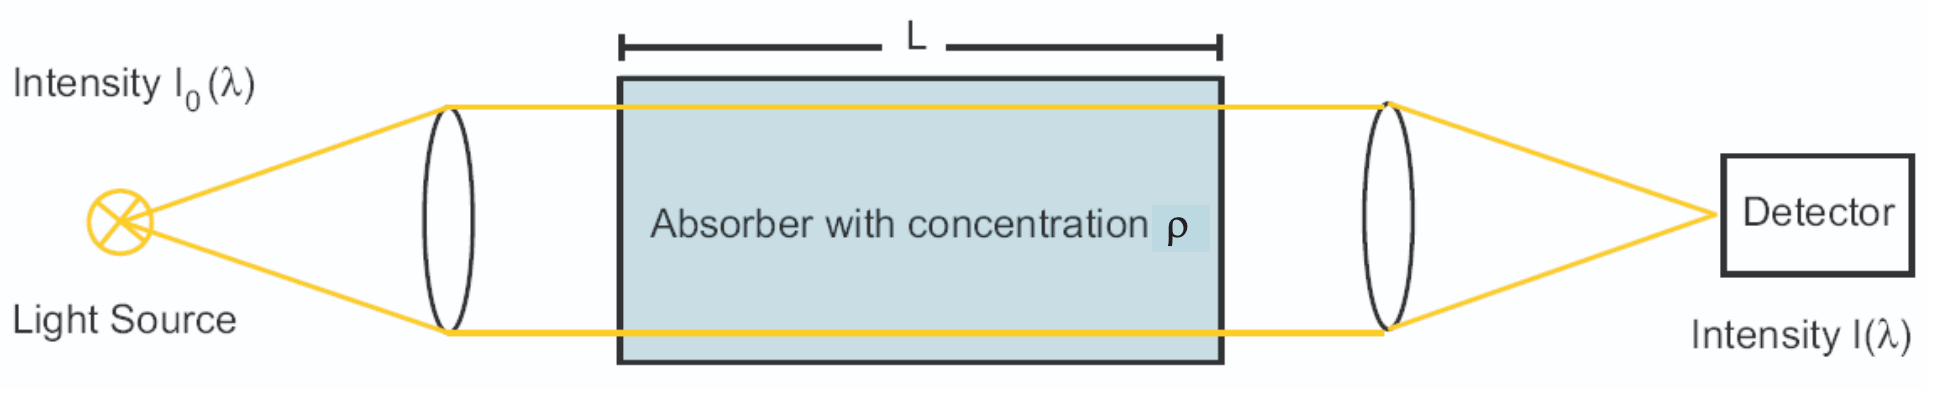
\includegraphics[width=\linewidth]{fig/lambert_beer.png}
    \captionof{figure}{Darstellung des Lambert-Beer Gesetzes}
	\label{fig:lambert-beer}
\end{center}

Die Größe des Verlustes kann mithilfe des Lambert-Beer Gesetzes bestimmt werden.
Sei $I_0 (\lambda)$ die Startintensität des Lichtstrahls, dann ist die Intensität $I(\lambda, L)$ nachdem der Lichtstrahl eine Länge $L$ der Mediums überwunden hat
    
\begin{align}
    I(\lambda, L) = I_0 (\lambda) \exp \left( - \rho L \sigma (\lambda)\right) ,\label{eq:lambert_beer_law}
\end{align}

wobei $\sigma (\lambda)$ der Absorptionswirkungsquerschnitt und $\rho$ die Konzentration des Spurengases ist.

\subsection{Kurzband Komponenten}\label{ssec:Kurzband}

\subsubsection{Fraunhofer Referenzspektrum}\label{sssec:fraunhofer_reference}

\subsubsection{Spurengas Absorption}\label{sssec:trace_gas_absorption}

Die Hauptmessgröße des DOAS is die \textit{slant column density} ($SCD$ oder $S$)
welche als die integrierte Dichte eines Spurengases $i$ entlang eines Lichtpfades der Länge $L$
    
\begin{align}
    SCD = S_i (\lambda) = \int_0^{L(\lambda)} \rho_i (s) \dd s ,\label{eq:SCD}
\end{align}

\subsection{Modifiziertes Lambert-Beer Gesetz}\label{ssec:mod_lamb-beer_law}

Wenn man nun diese Effekte mit einbezieht, so kann man ein neues modifiziertes Lambert-Beer Gesetz ausstellen.

\begin{align*}
    I(\lambda, L) = & I_0 (\lambda) \exp \left( -R ( \lambda ) - \sum_i \sigma_i (\lambda)
    S_i (\lambda) \right) \times \\
    & \exp \left[ - L \left( \sigma_{i0} (\lambda) \rho_o + \epsilon_R (\lambda) + \epsilon_M (\lambda) \right) \right], \label{eq:mod_lambert_beer_law}
\end{align*}

Die erste Exponentialfunktion beinhaltet alle Kurzband Effekte und die zweite alle Breitband Effekte.
Wenn man das modifizierte Lambert-Beer Gesetz nun nach $\log \frac{I}{I_0}$ umformt erhält man die optische Dichte $\tau$:

\begin{align}
\tau &= \log \frac{I}{I_0} \\
    &= - R(\lambda) - \sum_i \sigma_i (\lambda) S_i (\lambda) - \sum_k b_k \lambda^k,\label{eq:optical_density}
\end{align}

wobei das Polynom $\sum b_k \lambda^k$ für die Breitband Effekte zuständig ist.

\textcolor{red}{Brauchen wir noch mehr Grundlagen?}

\section{Versuchsdurchführung}\label{sec:versuchsdurchführung}

\subsection{Software kennenlernen}\label{get_to_know_the_software}

Während des Versuches wurde das Programm \verb*+DOASIS+ verwendet um die Spektren aufzunehmen und später die Fits durchzuführen.\\
Zu Beginn wurde durch variieren der Messzeit (\textit{exposure time}) und der Anzahl der Scans (\textit{exposures}) ein erster Überblick über das Programm \verb*+DOASIS+ verschafft.

\begin{center}
	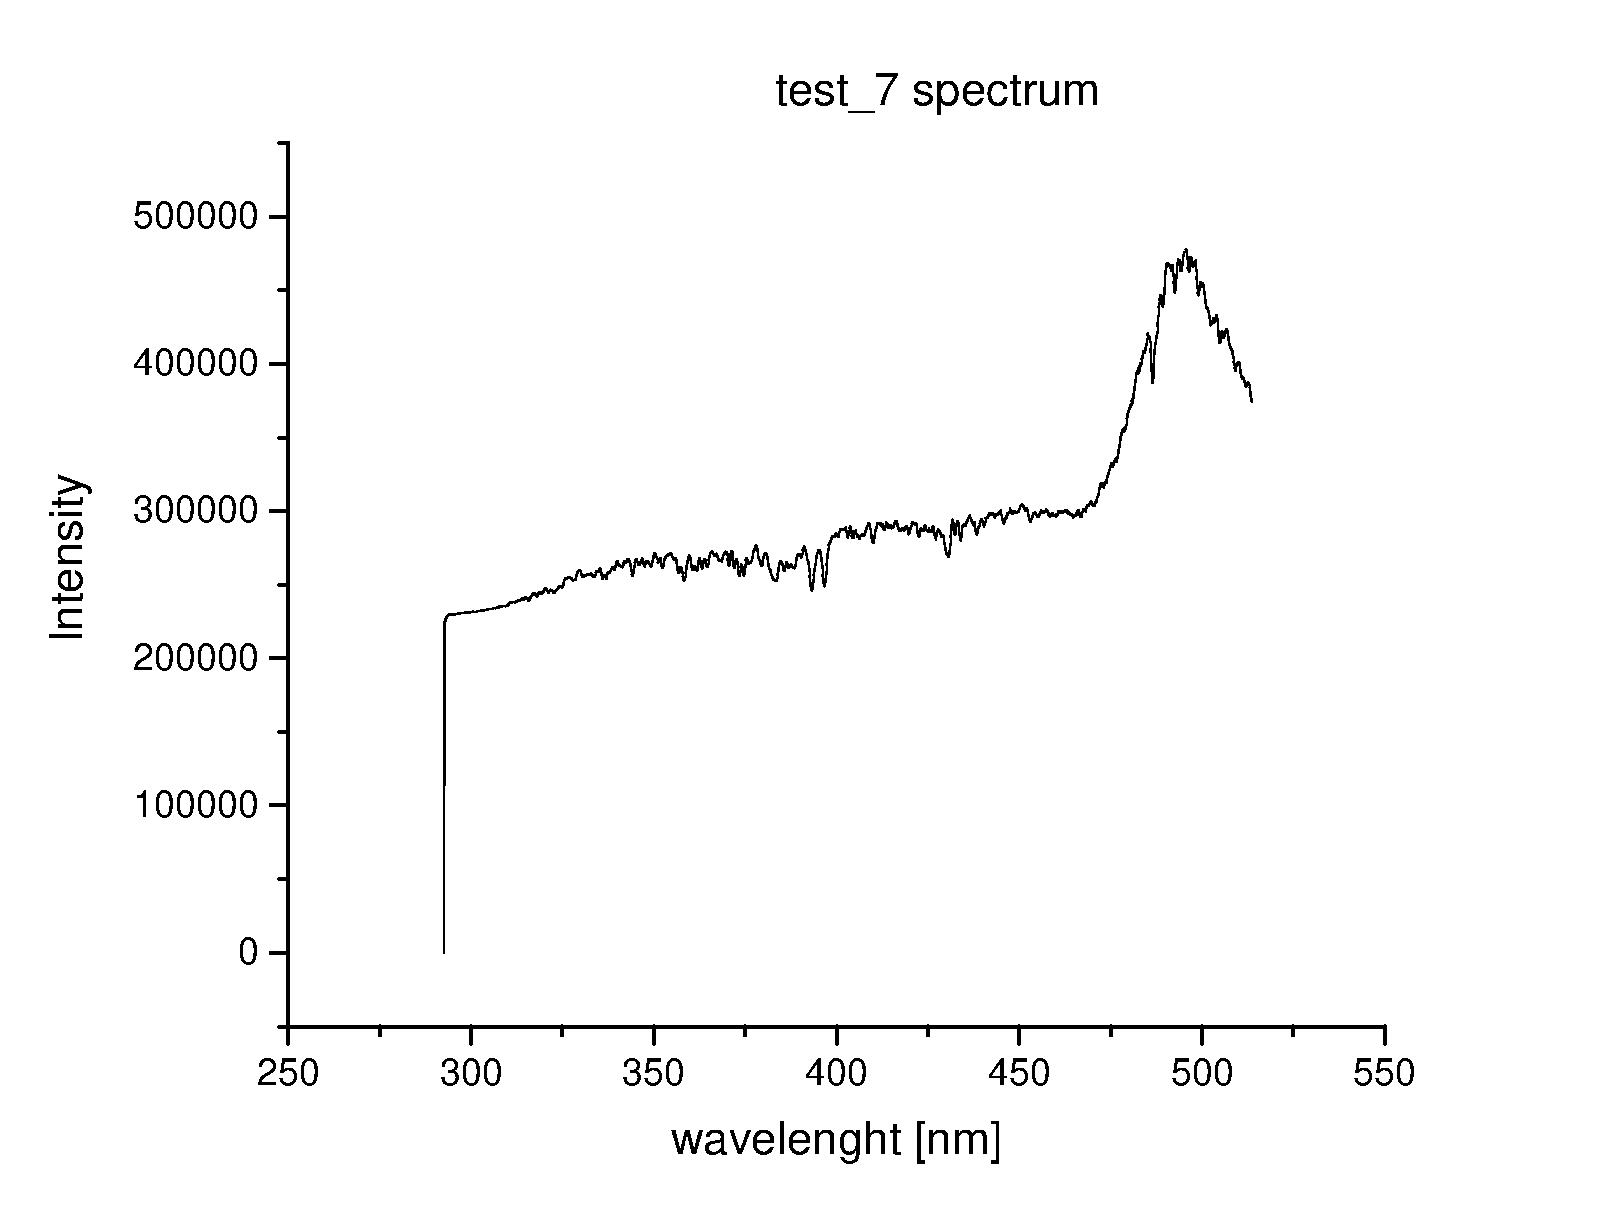
\includegraphics[width=\linewidth]{fig/test_7_spectrum.pdf}
    \captionof{figure}{Test Spektrum}
	\label{fig:test_spectrum}

\end{center}

\subsection{Charakterisierung der Messinstrumente}\label{ssec:characteristic_of_the_instruments}

\subsubsection{Offset und Dunkelstrom}\label{sssec:O&D}

Es gibt zwei Haupteffekte die Ungenauigkeiten bei der Messung verursachen können.
Durch Brownsche Bewegung in den Kabeln wird ein kleiner elektrischer Strom erzeugt, den man auch als Dunkelstrom bezeichnet.
Um die Größenordnung des Dunkelstromes einzuschätzen werden einminütige Messungen durchgeführt, bei denen die Kamera abgedeckt ist.\\
Die CCD-Kameras haben außerdem ein Offset, welcher durch viele kurze Messungen bestimmt werden kann.\\
Dunkelstrom und Offset müssen bei jedem folgenden Spektrum abgezogen werden.
Die Messung des Offsets wurde als erstes Durchgeführt. 
Hierbei wurden $20000$ Messungen mit jeweils $3$ \si{ms} Messzeit durchgeführt.
Anschließend wurde der Dunkelstrom bei verschiedenen Messzeiten gemessen (siehe Abbildung \ref{fig:dark_current}).
    
\begin{center}
	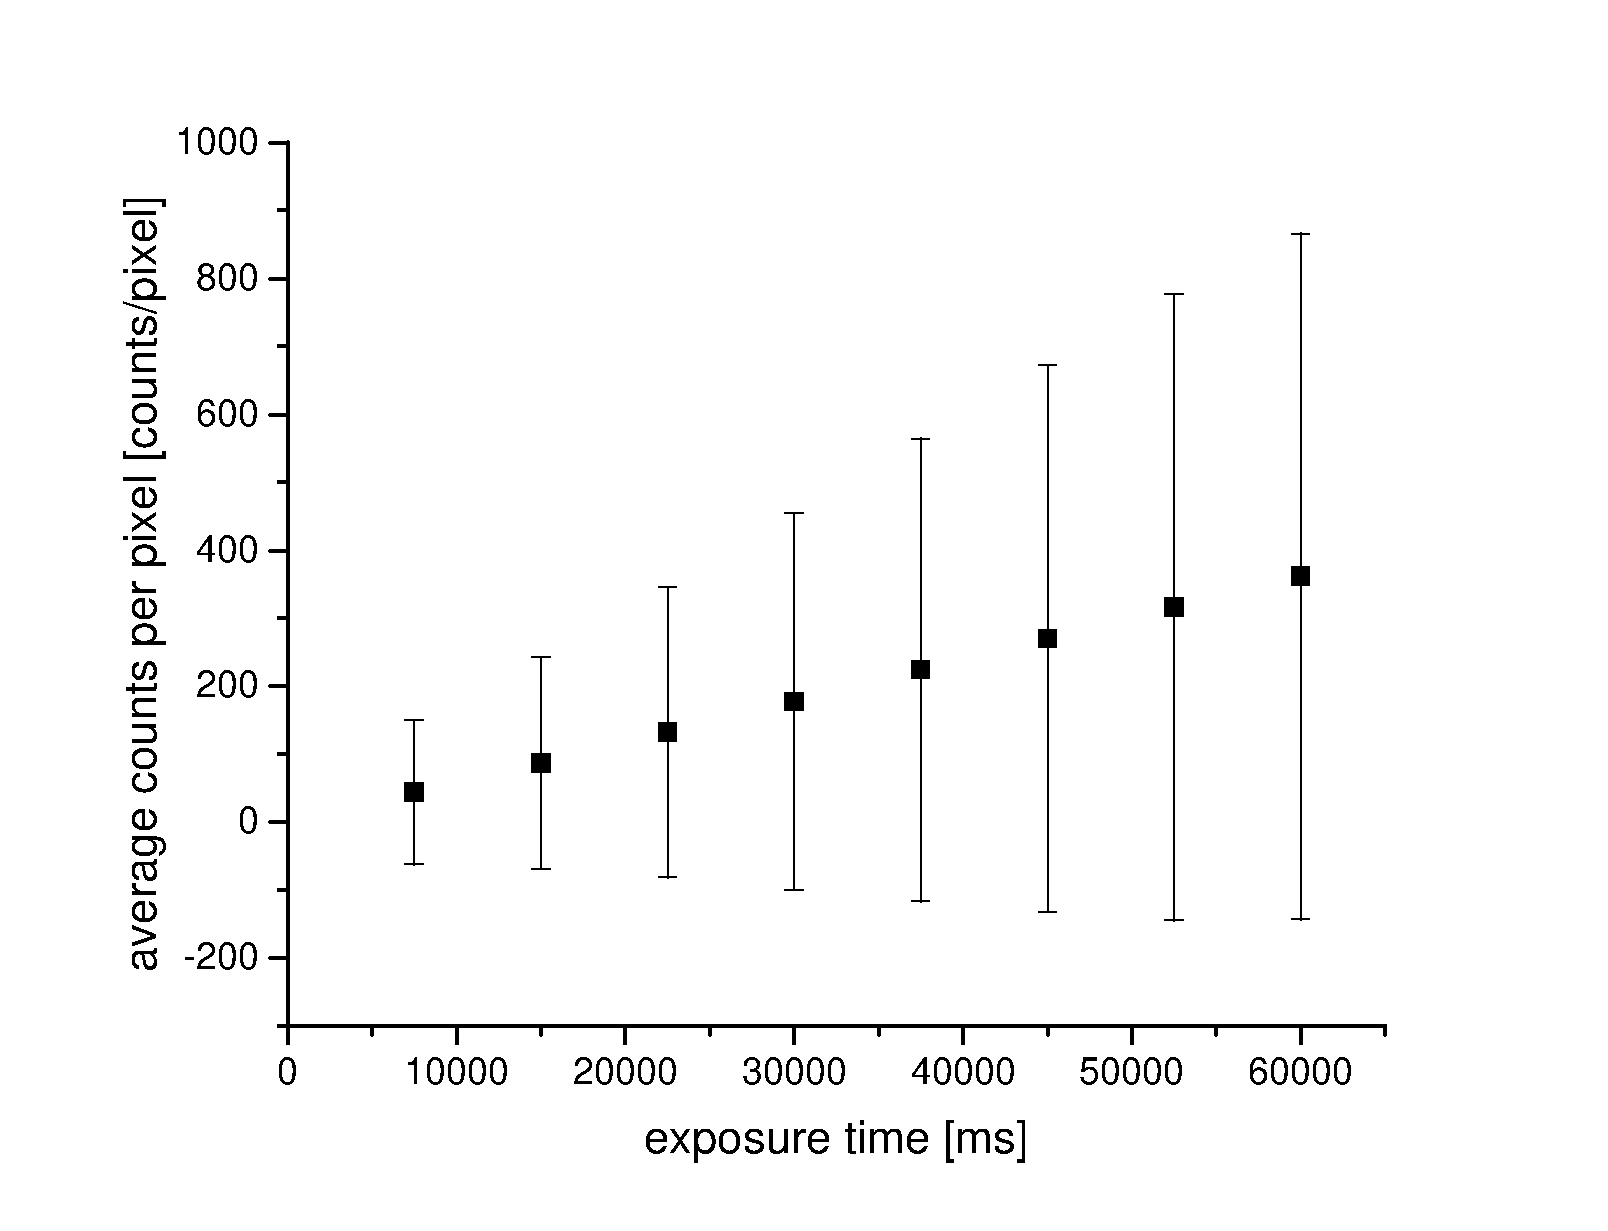
\includegraphics[width=\linewidth]{fig/dark_current_exposure_time_plot.pdf}
    \captionof{figure}{Abhängigkeit des Dunkelstromes von der Messzeit}
	\label{fig:dark_current}
\end{center}

\subsubsection{Instrumenten- und totales Rauschen}\label{sssec:instrumental_total_noise}

Wie im oberen Abschnitt \ref{sssec:O&D} gesehen, entstehen Messfehler, die zeitlich nicht konstant sind. Zunächst widmet man sich dem instrumentenbedingten Rauschen.
Dazu werden zwei Offsets mit identischen Einstellungen kurz hintereinander aufgenommen, über die entstandene Differenz ($\sigma_D$) lässt sich dann das Instrumentenrauschen bestimmen 

\begin{align}
\sigma_{I} = \frac{1}{\sqrt{2}}\sigma_D.\label{eq:instrumental_noise}
\end{align}

Ein Auftragen des Rauschens gegen die Anzahl der Scans liefert einen linearen Zusammenhang (siehe Diagramm \ref{fig:instrumental_noise})

\begin{center}
	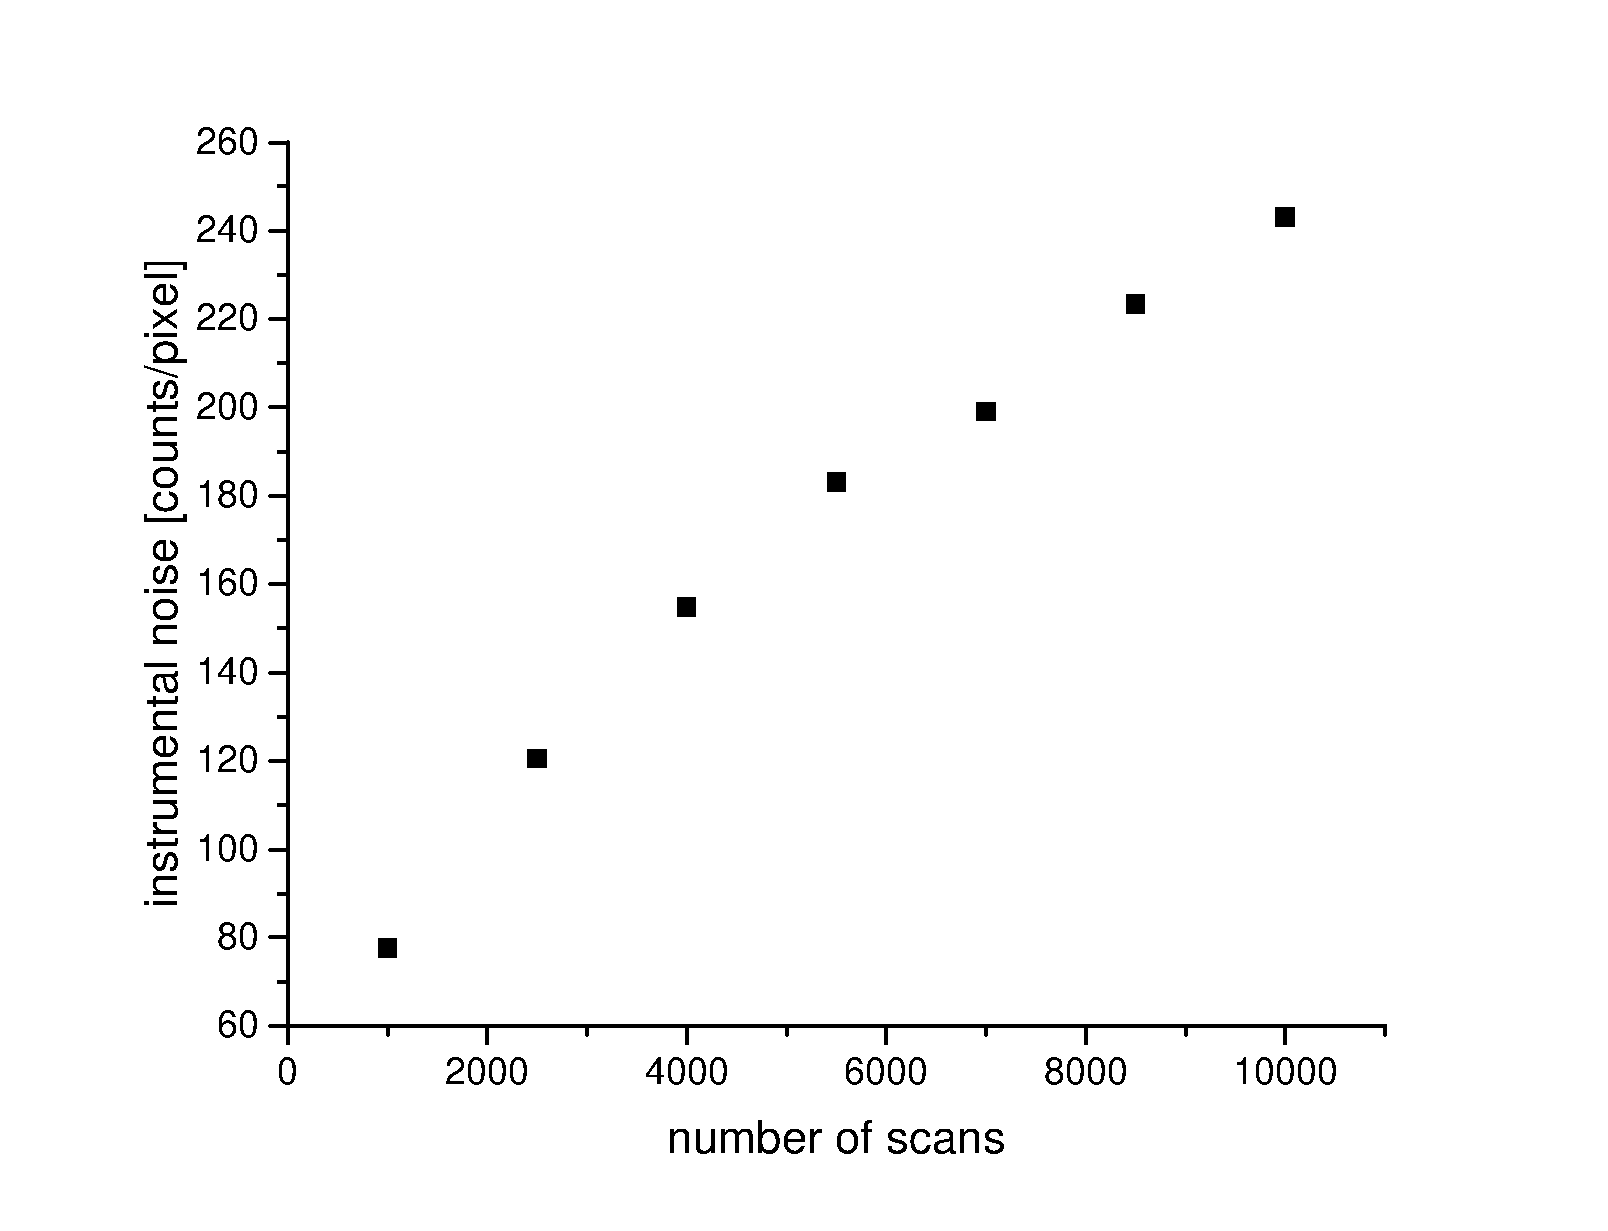
\includegraphics[width=\linewidth]{fig/instrumental_noise_diagramm.pdf}
	\captionof{figure}{Abhängigkeit des Instrumentenrauschens von der Anzahl der Scans}
	\label{fig:instrumental_noise}
\end{center}  

Zur Bestimmung des totalen Rauschens wurde nun das Spektrum einer Halogenlampe aufgenommen.
Es wurden ebenfalls wieder jeweils zwei Spektren bei identischen Einstellungen kurz hintereinander aufgenommen. 
Um systematische Strukturen, wie das Schwanken der Lampenintensität zwischen den beiden Messungen, zu berücksichtigen wurde ein Hochpassfilter an die Daten angelegt.

\begin{center}
	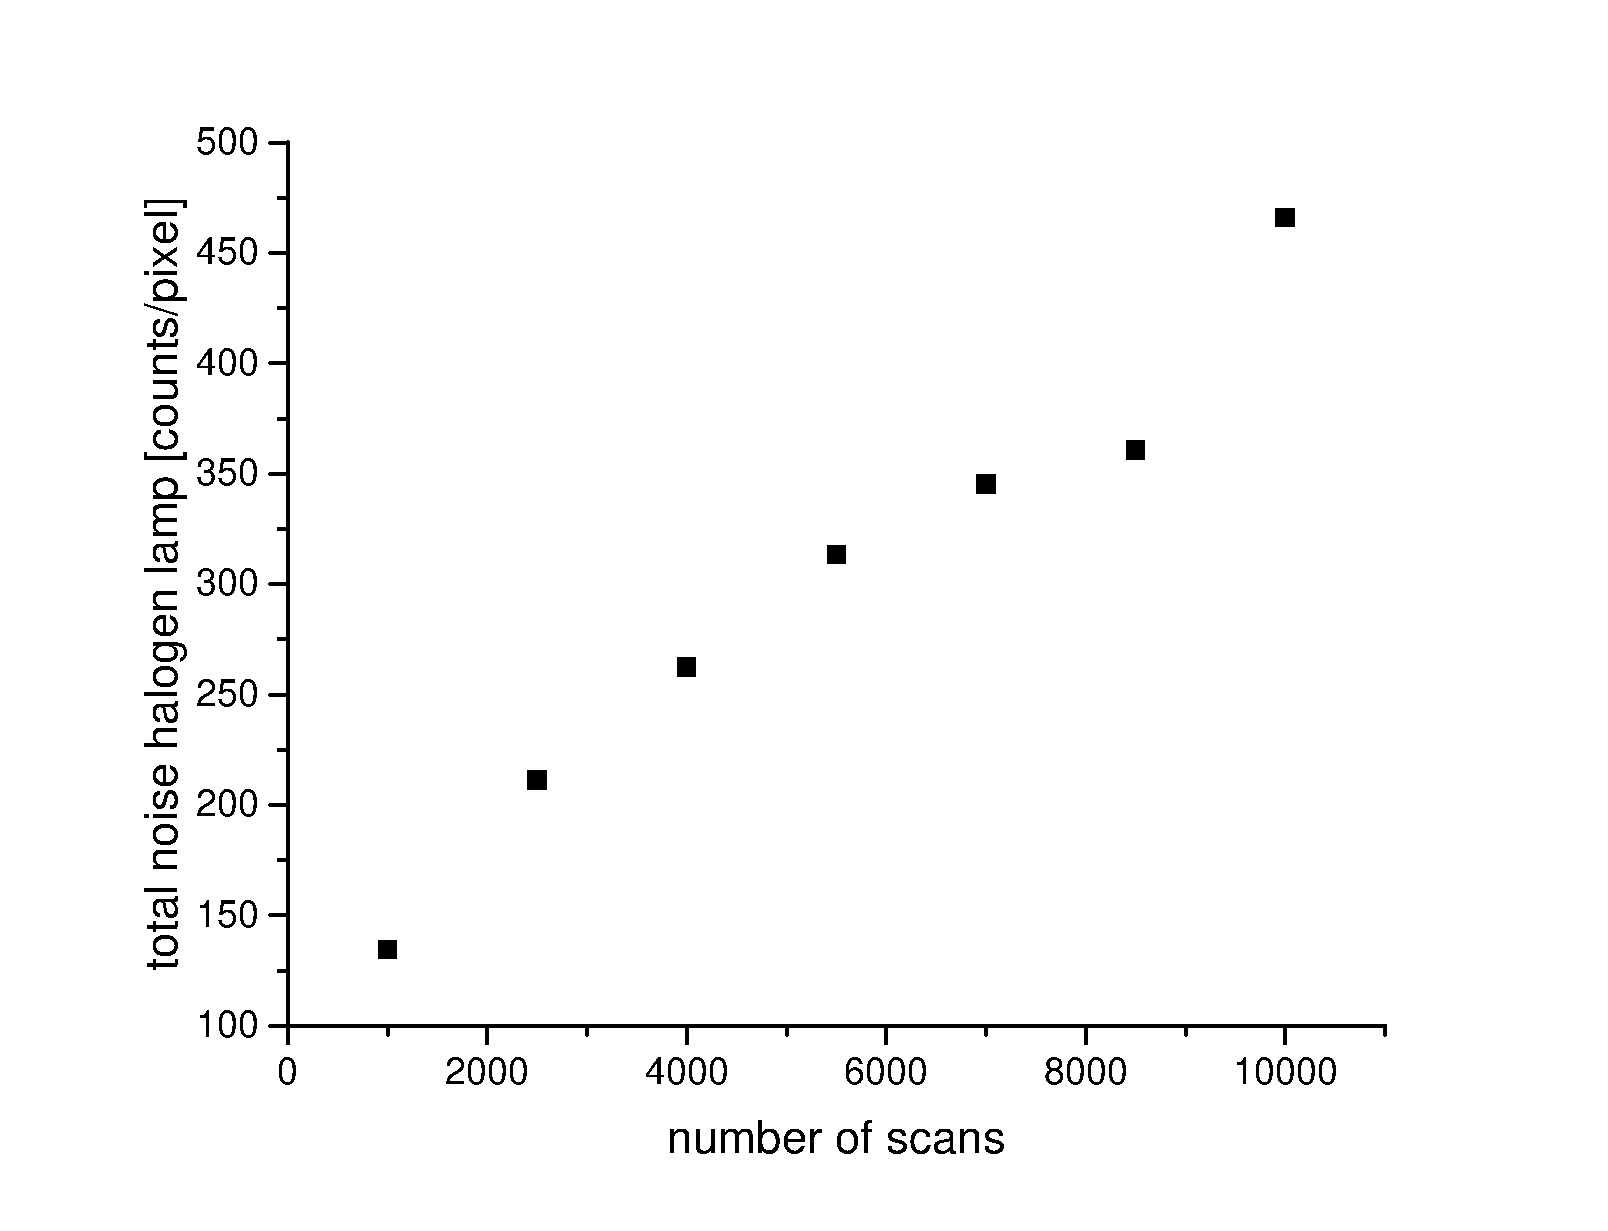
\includegraphics[width=\linewidth]{fig/total_noise_halogenlamp_plot.pdf}
	\captionof{figure}{Abhängigkeit des totalen Rauschens von der Anzahl der Scans}
	\label{fig:total_noise}
\end{center}  

Es zeigt sich in Abbildung \ref{fig:total_noise} die gleiche Charakteristik wie in Abbildung \ref{fig:instrumental_noise}. Lediglich die Stärke des Rauschen unterscheidet sich, was aber zu erwarten war, da im totalen Rauschen auch das Instrumentenrauschen integriert ist.
\\
Eine weitere Untersuchung der Halogenlampenspektren ermöglicht einen Einblick in die optische Dichte des relativen totalen Rauschens. Dazu wurden die zuvor aufgenommenen Spektren durcheinander geteilt und anschließend der Logarithmus des Ergebnisses betrachtet.
\\
\textcolor{red}{Hier brauchen wir eines der Bilder log\_nummer.sp2}
\\
Man erwartet, dass der Mittelwert bei Null liegt, da zwischen der Aufnahme der Spektren so wenig wie möglich Zeit vergangen ist. Allerdings kann bei kleinerer Channelzahl höhere Schwankungen ausgemacht werden und insgesamt ist ein kurven artiger Verlauf zu erkennen.
Das größere Schwanken lässt sich darauf zurückführen, dass bei kleiner Channelzahl die \textit{Counts} geringer ausfallen als bei höherer Channelzahl.
Durch Schwankungen der Halogenlampenintensität ensteht in den Daten die beobachtete Krümmung, welche bei höherer Scanzahl größer wird. Die Schwankungen verlieren bei höheren \textit{Counts} an Bedeutung.

\subsubsection{Kalibrierung des Spektrometers}\label{sssec:calibrating_the_spectrometer}

Zur Kalibrierung des Spektrometers wird eine Quecksilberdampflampe verwendet, da diese gut zu identifizierende Spektrallinien aufweist.
Das aufgenommene Spektrum wurde nach bekannten Spektrallinien untersucht und anhand von vier Maxima (entprechend den Channelnummern: 335, 595, 946, 1239) das Spektrometer kalibriert. 

Für die Kalibrierung wird ein Polynom zweiter Ordnung genutzt mit folgenden Parameter: 

\begin{align}
	coeff_0 &= 292.61 \pm 0.043611\\
	coeff_1 &= 0.12726 \pm 0.00016266\\
	coeff_2 &= 9.3859 \cdot 10^{-6} \pm 1.193 \cdot 10^{-7} 
\end{align}
 
Über die \textit{full width at half max}(FWHM) lässt sich nun die optische Auflösung des Spektrometers bestimmen.

\begin{center}
	
\begin{tabular*}{\linewidth}{@{\extracolsep{\fill}} c c c}
	\toprule
	Maximum & Channel & FWHM [\si{nm}] \\
	\midrule
	1 & $\sim 160$ & $1.2 \pm 0.1$ \\
	2 & $\sim 594$ & $0.8 \pm 0.1$ \\
	3 & $\sim 945$ & $0.6 \pm 0.1$ \\
	4 & $\sim 1240$ & $0.7 \pm 0.1$ \\
	\bottomrule
\end{tabular*}

	\captionof{table}{Optische Auflösung der verschiedenen Maxima} %\cite{atm_components}
	\label{fig:optical_resolution}
\end{center}

Bei der Analyse der FWHM stellt sich heraus, dass die optische Auflösung des Spektrometers bei höherer Channelzahl besser wird, deshalb wird versucht in den folgenden Messungen die Analyse, wenn möglich, im hohen Channelbereich durchzuführen.

\subsection{Labormessungen}\label{ssec:Labormessungen}

\subsubsection{Anpassung von Referenzspektren}\label{sssec:convolution_of_reference}

Mithilfe eines Literaturspektrums kann ein Vergleichsspektrum generiert werden. 
Die verwendeten Literaturspektren haben allerdings unterschiedliche Auflösungen und daher muss man diese entsprechend skalieren.
Dies kann mithilfe einer Faltung erledigt werden.
Die Faltung einer Funktion $f$ mit einer Funktion $g$ ist definiert als

\begin{align}
    (f \ast g) (x) := \int f(y) g(x-y) \dd y .
\end{align}

Die Faltung sorgt zusätzlich dafür, dass das Spektrum geglättet wird.
Wellenlänge die außerhalb des Bereiches der Messgeräte liegt werden durch die Faltung abgeschnitten.\\
Es wurden Spektren von  \ch{CO2}, \ch{H2O}, \ch{O3} und \ch{O4} angepasst.
Bei dem Referenzspektrum von \ch{H2O} wurde ,im Gegensatz zu den anderen Spektren, das Spektrum erweitert. Dafür wurden um die Struktur Nullwerte eingefügt. \textcolor{red}{Klingt blöd}
 
\subsubsection{\ch{NO2} Spektrum von einer gefüllten Gaszelle}\label{sssec:lab_no2_spectra}

Um die in den vorigen Abschnitten durchgeführten Vorbereitungen zu testen wird das Spektrum der Halogenlampe untersucht, wenn eine Glasküvette mit \ch{NO2} gefüllt in den Lichtweg gestellt wird.
\textcolor{red}{Vielleicht hier Bild oder Sketch vom Versuchsaufbau}

Mithilfe des Lambert-Beer Gesetztes lässt sich nun über die optische Dichte innerhalb der Gasküvette die Konzetration bestimmen (vgl. Gleichung \eqref{eq:lambert_beer_law} und \eqref{eq:optical_density})

\begin{align}
\tau = \ln(\frac{I_0(\lambda)}{I(\lambda)}) = \sigma_{\ch{NO2}}(\lambda) \cdot \rho_{\ch{NO2}} \cdot L.
\end{align}

Bei der Aufnahme der Spektren ist drauf zu achten, dass kein Teilbereich in Sättigung ist. Ein mögliches Anpassen der Einstellungen der Messungen ist ohne weiteres Möglich. Eine Änderung der Anzahl der Scans oder der Sättigung macht sich nur als eine Konstante bemerkbar, die im 
\textcolor{red}{ergänzen warum Änderungen nichts ausmachen}

Über einen \textit{least-square-fit} wird nun die SCD so variiert, sodass das $\chi^2$ minimiert wird. In \ref{fig:different_fit_ranges} wurden die Fitparameter bei verschiedenen Fitbereichen betrachtet. Dabei wurde immer ein Polynom 5. Grades ohne Offset gefittet.
Den optimalen Fitbereich lässt sich über ein Überlagerung (siehe Abbildung \ref{fig:range_search}) des aufgenommenen Spektrums mit dem \ch{NO2} Referenzspektrum finden.

\begin{center}
	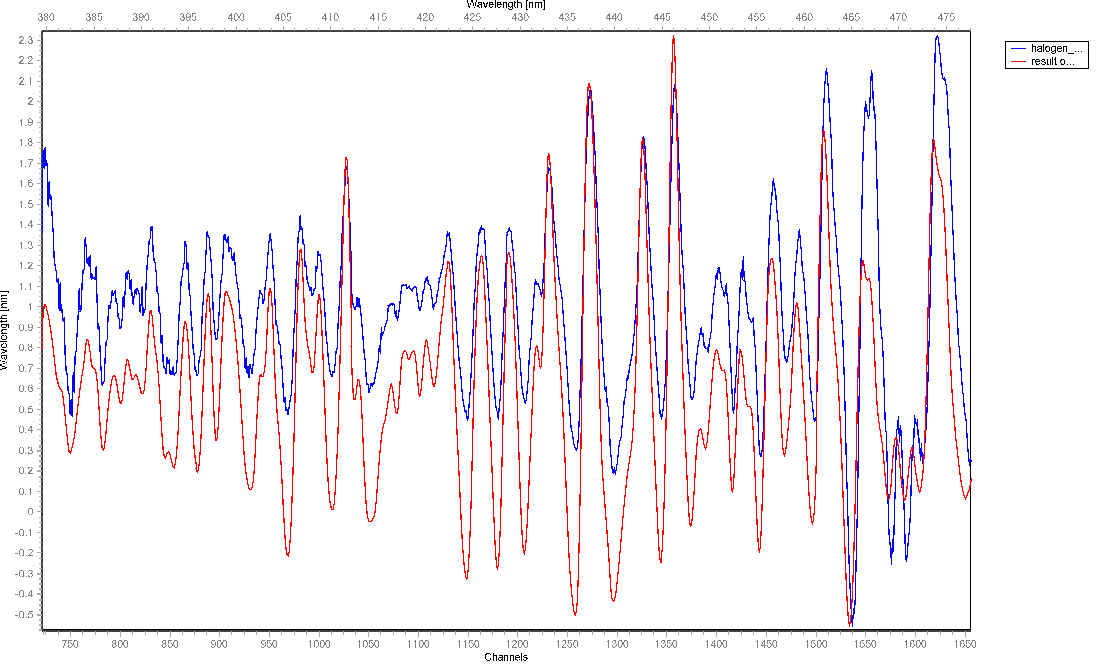
\includegraphics[width=\linewidth]{fig/range_search_test.png}
	\captionof{figure}{Überlagerung des aufgenommenen und des Referenz- Spektrums}
	\label{fig:range_search}
\end{center}

Die Überlagerung zeigt im Channelbereich $1000-1700$ die gleichen Strukturen. Der Fit wird in diesem Berich durchgeführt.
Für die genau Bestimmung der \ch{NO2} Konzentration wurde ein Channelbereich von $1206-1663$ ausgewählt, dabei wurde darauf geachtet, dass die die Intensität bei einer Wellenlänge von $470$\si{nm} ca. $80$\% betrug.
Damit konnten beim Fit die Parameter

\begin{align}
	\chi^2 &= 4.367 \cdot 10^{-3},\\
	fit coeff &= -4.96 \cdot 10^{17} \pm 1.95 \cdot 10^{15},\\
	shift &= 0.0955 \pm 0.00538,\\
	squeeze &= 0.993 \pm 0.000159, 
\end{align}

erreicht werden.
Mit der nun bestimmten \textit{slant column density} kann nun die \ch{NO2} Konzentration in der Küvette berechnet werden.
Die Länge wurde von Hand auf $2.0 \pm 0.1$\si{cm} bestimmt, sodass sich mit der Gaußschen Fehlerfortpflanzung eine Konzentration von

\begin{align}
	\rho_{\ch{NO2}} = (2.48 \pm 0.12) \cdot 10^{20} \Bigl[ \frac{\text{molecules}}{\si{liter}}\Bigr]
\end{align}

ergibt.	
Ebenfalls lässt sich nun das Mischverhältnis auf

\begin{align}
	R = \frac{\rho_{\ch{NO2}}}{\rho_{std.}} = (9.22 \pm 0.45) *10^{-3}
\end{align}

beziffern. Dazu wurde für die $\rho_{std.}$ aus den Normalbedingungen gewonnen.

\begin{align}
	\rho_{std.} = \frac{N_A}{V_M}.
\end{align}
 	
Mit $N_A = 6.022 \cdot 10^{23} \frac{1}{\si{mol}}$ und $V_M = 22.4 \frac{\si{liter}}{\si{mol}}$.

\subsection{Atmosphärische Messungen}\label{ssec:atmospheric_measurements}

Nachdem man sich nun mit dem Messverfahren und der Analyse der Daten vertraut gemacht hat, werden nun atmosphärische Spurengase untersucht. In diesem Praktikumsversuch beschränkt man sich auf \ch{O3} und \ch{NO2}.
Für die Analyse wurde ein Tag ausgesucht, bei dem gutes Wetter herrschte, sodass Wolken nicht die Messung beeinträchtigen können, über einen langen Zeitraum aufgenommen wurde, sowie nicht zu weit in der Vergangenheit lag, da man einer möglichen Abweichung von Dunkelstrom und Offset minimieren wollte.
Die Wahl fiel auf den 23.04.2019, wo über einen Zeitraum von $9:13 - 23:56$ UTC aufgenommen wurde.

\subsubsection{Optimierung des Fitalgorithmuses}\label{sssec:configure_fit}

Die für die \verb*+DOASIS+ nötige Referenzmessung, die Fraunhoferreferenz, wurde die Tagesmessung mit dem niedrigsten
\textit{solar zenith angle} (SZA) ausgewählt. Da der statistische Lichtweg hier am kürzesten ist und somit am wenigsten von möglichen Spurengasen absorbiert wurde.
Um nun die Parameter des Fits optimal anpassen zu können, wird ein Spektrum bei $80$ SZA ausgewählt um die größtmögliche Differenz zwischen den beiden Spektren zu erzeugen. Dies gewährleistet, dass die zu untersuchenden Strukturen am prägnantesten hervortreten.
\\
Aufgrund des inelastischen \textit{rotational Raman scattering} kommt es zu leichten Wellenlängenverschiebungen, dies sorgt für eine Art \textit{Auffüllung} der starken Absorptionslinien.
Um dies Vorzubeugen wird ein \textit{Ringspektrum} $R(\lambda)$ aus dem Fraunhoferspektrum berechnet.
Aus einer Berechnung der optischen Dichte und dem Vergleich mit den Referenzspektren der Spurengase (vgl. Abschnitt \ref{sssec:lab_no2_spectra}) werden die jeweiligen Fitbereiche ermittelt. Die Fitbereiche sind in Tabelle \ref{fig:fit_of_atmospheric_data} aufgelistet.
\\
Der Fitalgorithmus greift nun auf das Fraunhoferreferenzspektrum als first fit reference, dem Ringspektrum und den Referenzwirkungsquerschnitten der Spurengase zurück. \ch{H20} konnte dabei nicht immer verwendet werden, da es in manchen Bereichen Singularitäten aufweist.
\textcolor{red}{Wirkungsquerschnitte? muss einheitlich sein. Danach noch präzisieren starr manche}

\subsubsection{Untersuchung der Tagesmessung}

Nachdem die Fitbereiche optimiert wurde, werden die die Daten des ganzen Tages untersucht. Dabei standen 436 Aufnahmen zur Verfügung.

\begin{center}
	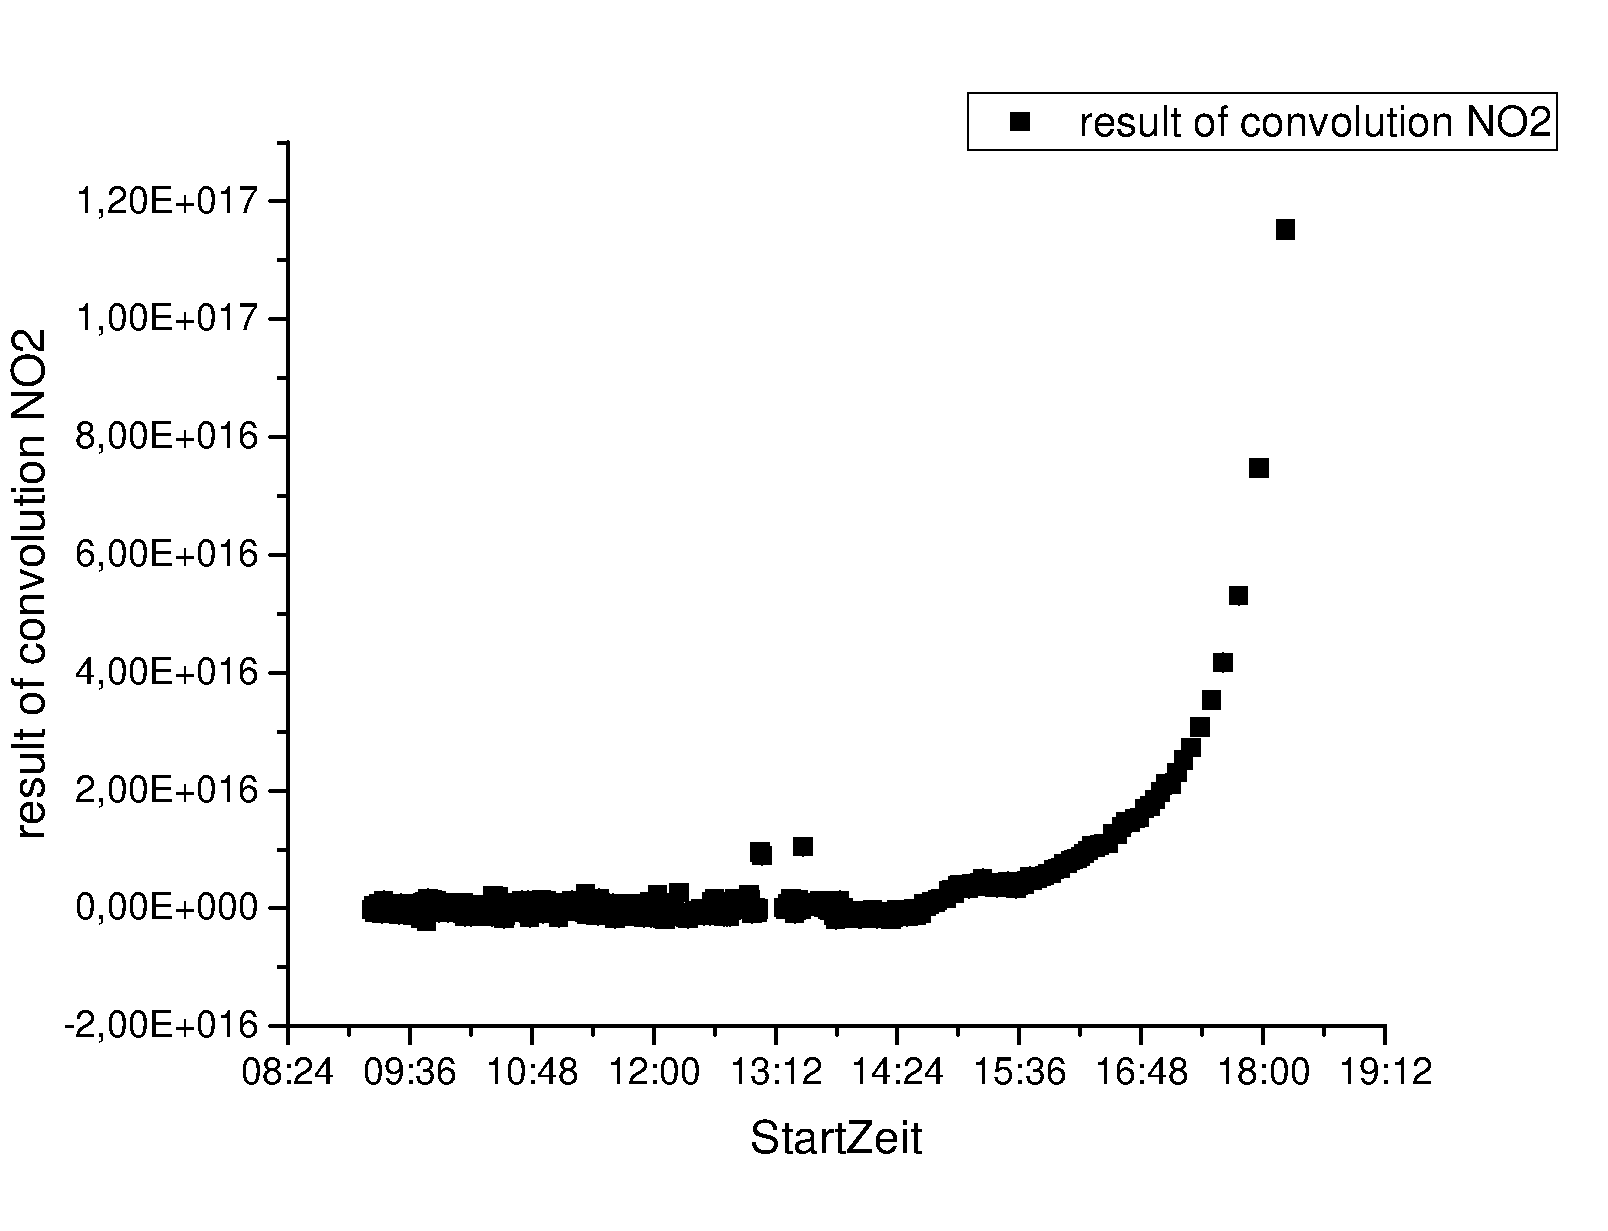
\includegraphics[width=\linewidth]{fig/SCD_Time_Plot_NO2.pdf}
	\captionof{figure}{$\delta$SCD von \ch{NO2} über den Tag des 24.04.2019}
	\label{fig:delta_SCD_time_NO2}
\end{center}
       
\begin{center}
	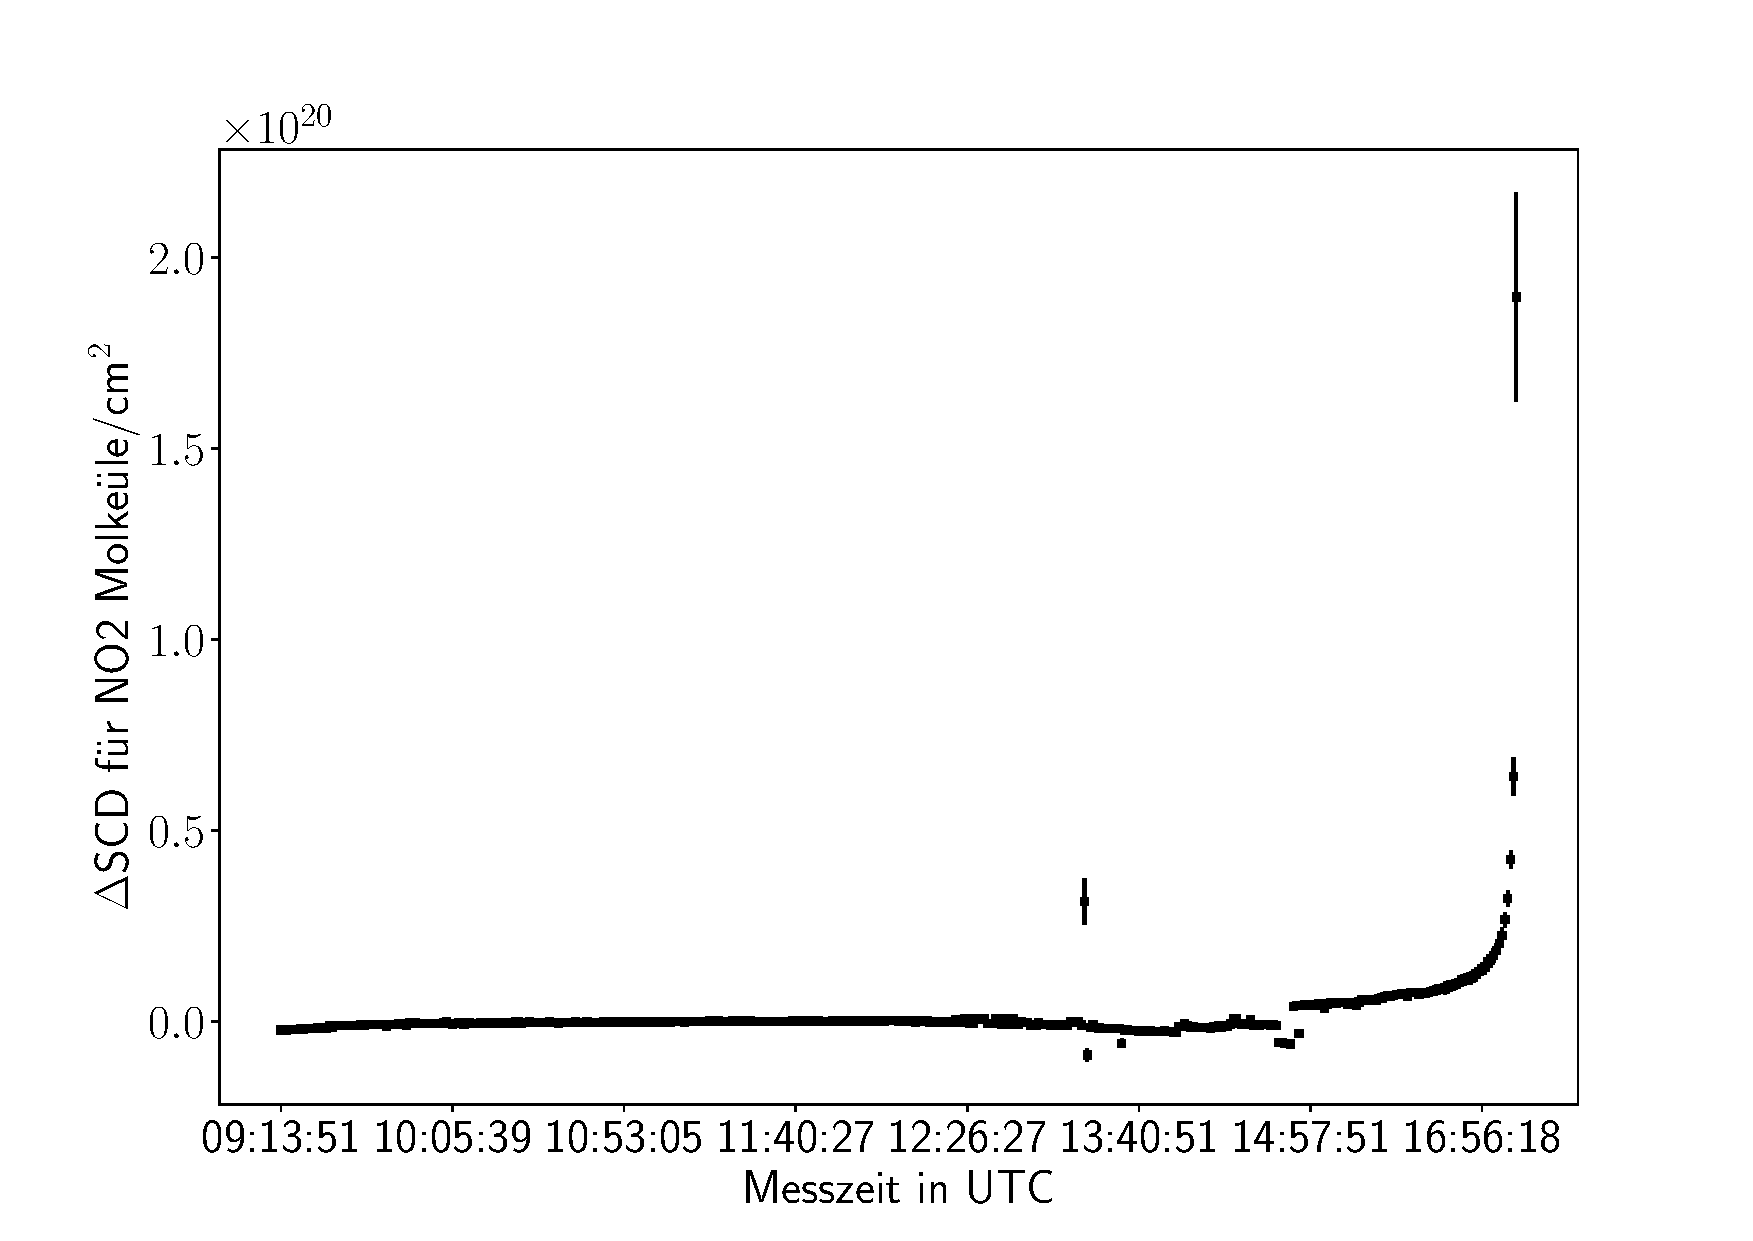
\includegraphics[width=\linewidth]{fig/SCD_Time_Plot_O3.pdf}
	\captionof{figure}{$\delta$SCD von \ch{O3} über den Tag des 24.04.2019}
	\label{fig:Delta_SCD_time_O3}
\end{center}       

\textit{Warum die so aussehen}

Eine Untersuchung der SCD gegen den \textit{Air Mass Factor}(AMF), lässt Rückschlüsse über eine Konzentrationsänderung über den Tag zu.

\begin{center}
	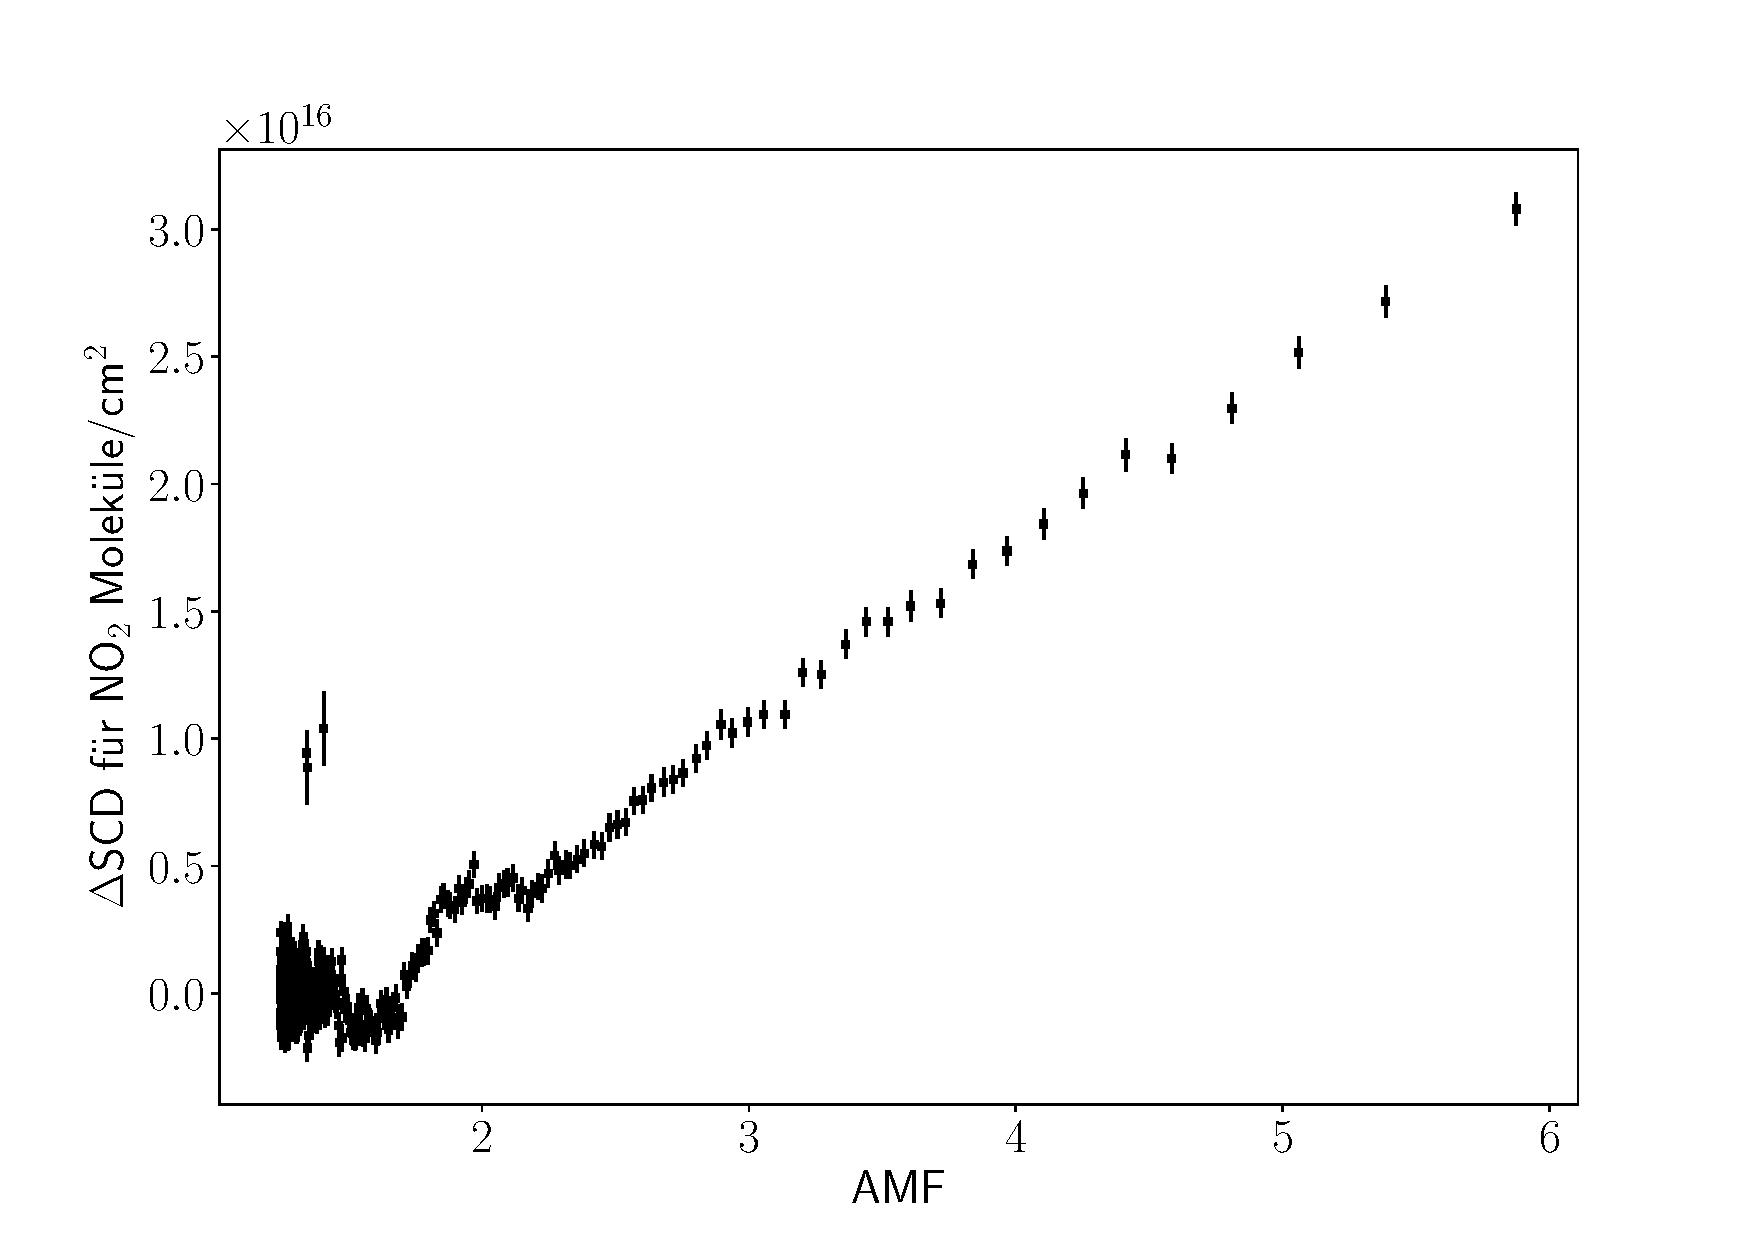
\includegraphics[width=\linewidth]{fig/Langley_Plot_NO2_cut.pdf}
	\captionof{figure}{Langley-Plot von \ch{NO2}}
	\label{fig:langley_NO2}
\end{center}

\begin{center}
	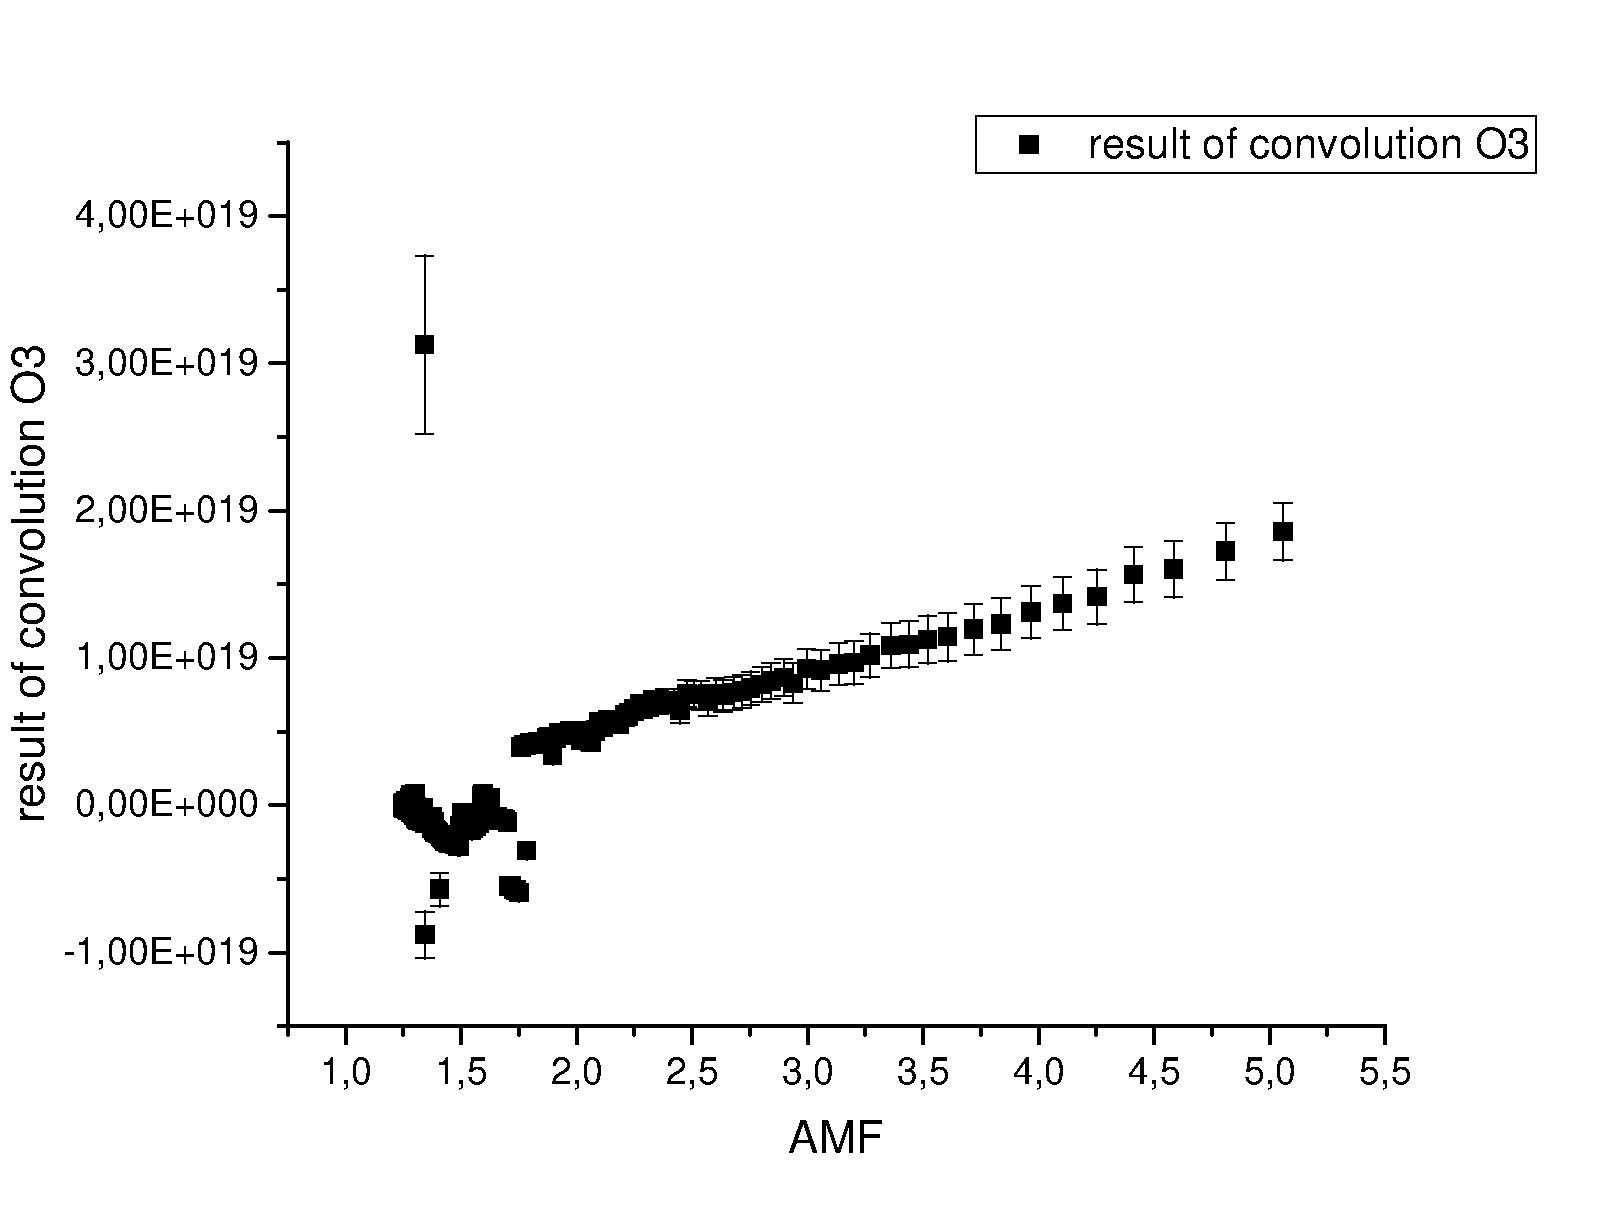
\includegraphics[width=\linewidth]{fig/Langley_Plot_O3_cut.pdf}
	\captionof{figure}{Langley-Plot von \ch{O3}}
	\label{fig:langley_O3}
\end{center}

\textcolor{red}{Erklärung usw., außerdem Fit für $\text{SCD}_ref$ von \ch{O3}}

Eine Veranschaulichung der Konstanz \textcolor{red}{?} von  \ch{O3} lässt sich über die \textit{vertical column density}(VCD) aufzeigen.
\\
\textcolor{red}{Hier dann der Plot, wir haben es bisher leider gegen das Falsche aufgetragen}
\\
Die VCD berechnet sich dabei leicht über geometrische Zusammenhänge: 

\begin{align}
	VCD = SCD \cdot \cos(\theta)
\end{align}

\textcolor{red}{Vergleich mit Daten von Satellitenmessungen}

\subsection{Multi Axis DOAS}\label{ssec:multi_axis_DOAS}

Einen Einblick in die vertikale Verteilung der Spurengase liefert die MAX-DOASIS Methode.
Es wurden vier Messreihen aufgenommen, die jeweils Messungen bei $7\circ,12\circ \text{und} 90\circ$ beinhalten. Dabei wurde immer beim kleinsten Winkel angefangen.
Die Messung wurde bei starker Bewölkung von 14:41 bis 15:01 MEZ durchgeführt.
Der Fit von \ch{O4} wurde im Channelbereich von $1500-1800$ durchgeführt, wobei dieser Bereich bei einigen Messungen angepasst werden musste. Dies war wie folgt der Fall $1.\text{Messung}:1550-1750, 2.\text{Messung}:1550-1720, 4.\text{Messung}:1550-1750, 5.\text{Messung}:1550-1750$.
Die Fitergebnisse sind in Tabelle \ref{fig:fit_multi_axis_DOAS} aufgetragen.
Eine $\delta$SCD Analyse der Daten erlaubt uns nun die oben erwähnte vertikale Verteilung der Gase zu untersuchen.
\\
\textcolor{red}{Hier die Plots, welche Gase in Troposphäre, Wolken?, usw.}
\\

\section{Diskussion}\label{sec:discussion}


\end{multicols}

\newpage

\appendix

\section{Tabellen}\label{tables}
\newcolumntype{d}[1]{D{.}{.}{3.1}}
\begin{center}
	
	\begin{tabular*}{\linewidth}{@{\extracolsep{\fill}} c d{1} c}
		\toprule
		Belichtungszeit [\si{ms}] & \multicolumn{1}{c}{Mittelwert [$\frac{\text{counts}}{\text{pixel}}$]} & Standardabweichung [$\frac{\text{counts}}{\text{pixel}}$] \\
		52500 & $316.0$ & $460.9$ \\
		45000 & $270.2$ & $401.9$ \\
		37500 & $223.9$ & $340.7$ \\
		30000 & $177.8$ & $277.0$ \\
		22500 & $132.1$ & $213.4$ \\
		15000 & $87.2$ & $155.6$ \\
		7500 &  $43.3$ & $105.9$ \\
		\bottomrule
	\end{tabular*}
	
	\captionof{table}{Dunkelstrom bei unterschiedlichen Belichtungszeiten} 
	\label{fig:dark_current_exposure_time}
\end{center}

\vspace{2cm}

\begin{center}
	
	\begin{tabular*}{\linewidth}{@{\extracolsep{\fill}} c c c}
		\toprule
		Anzahl der Scans & Mittelwert [$\frac{\text{counts}}{\text{pixel}}$] & Standardabweichung [$\frac{\text{counts}}{\text{pixel}}$] \\
		\midrule
		10000 & $-1112.8$ & $343.6$ \\
		8500 & $-1107.8$ & $315.9$ \\
		7000 & $-444.5$ & $281.4$ \\
		5500 & $109.1$ & $258.9$ \\
		4000 & $-147.9$ & $219.1$ \\
		2500 & $-188.7$ & $170.5$ \\
		1000 &  $-8.7$ & $109.6$ \\
		\bottomrule
	\end{tabular*}
	
	\captionof{table}{Differenz Offset bei unterschiedlicher Scanzahl} 
	\label{fig:difference_offset}
\end{center}

\vspace{2cm}

\begin{center}
	
	\begin{tabular*}{\linewidth}{@{\extracolsep{\fill}} c c c}
		\toprule
		Anzahl der Scans & Mittelwert [$\frac{\text{counts}}{\text{pixel}}\cdot 10^{-15}$] & Standardabweichung [$\frac{\text{counts}}{\text{pixel}}$] \\
		\midrule
		10000 & $47$ & $658.8$ \\
		8500 & $170$ & $538.3$ \\
		7000 & $29$ & $488.3$ \\
		5500 & $94$ & $443.0$ \\
		4000 & $-49$ & $371.2$ \\
		2500 & $-9.5$ & $299.0$ \\
		1000 &  $3.3$ & $190.1$ \\
		\bottomrule
	\end{tabular*}
	
	\captionof{table}{Differenz Offset bei unterschiedlicher Scanzahl (Halogen)} 
	\label{fig:difference_offset_halogen}
\end{center}

\vspace{2cm}

\begin{center}
	
	\begin{tabular*}{\linewidth}{@{\extracolsep{\fill}} c c c c}
		\toprule
		Maximum & Channel & Maximum [$\frac{\text{counts}}{\text{pixel}}$] & FWHM [\si{nm}]\\
		\midrule
		1 & $\sim 160$ & $635.8$ & $1.2 \pm 0.1$\\
		2 & $\sim 594$ & $920.0$ & $0.8 \pm 0.1$\\
		3 & $\sim 945$ & $1150.5$ & $0.7 \pm 0.1$ \\
		4 & $\sim 1240$ & $3612.3$ & $0.7 \pm 0.1$ \\
		\bottomrule
	\end{tabular*}
	
	\captionof{table}{Maxima des Quechsilberdampfspektrums (unkalibriert)} 
	\label{fig:max_mercury_uncalibrated}
	
\end{center}

\vspace{2cm}

\begin{center}
	
	\begin{tabular*}{\linewidth}{@{\extracolsep{\fill}} c c c}
		\toprule
		Maximum & Channel & FWHM [\si{nm}] \\
		\midrule
		1 & $\sim 160$ & $1.2 \pm 0.1$ \\
		2 & $\sim 594$ & $0.8 \pm 0.1$ \\
		3 & $\sim 945$ & $0.6 \pm 0.1$ \\
		4 & $\sim 1240$ & $0.7 \pm 0.1$ \\
		\bottomrule
	\end{tabular*}
	
	\captionof{table}{Optische Auflösung der verschiedenen Maxima} %\cite{atm_components}
	\label{fig:optical_resolution}
\end{center}

\vspace{2cm}

\begin{center}
	
	\begin{tabular*}{\linewidth}{@{\extracolsep{\fill}} c c c c c}
		\toprule
		Bereich &$\chi^{2}\cdot 10^{-4}$ & \multicolumn{1}{c}{Fit coeff. $\cdot 10^{15}$} & shift & squeeze \\
		\midrule
		$1150-1379$ & $8.67$ & $-484 \pm 1.97$ & $-0.00497 \pm 0.00495$ & $0.994 \pm 0.000333$ \\
		$1026-1377$ & $19.2$ & $-472 \pm 2.08$ & $0.0533 \pm 0.00682$ & $0.955 \pm 0.000261$\\
		$1026-1496$ & $33.2$ & $-475 \pm 2.23$ & $0.052 \pm 0.00682$ & $0.995 \pm 0.000246$ \\
		$1026-1663$ & $43.7$ & $-488 \pm 1.95$ & $0.091 \pm 0.00546$ & $0.993 \pm 0.000162$\\
		\bottomrule
	\end{tabular*}
	
	\captionof{table}{Fit bei verschiedenen  Fitbereichen}
	\label{fig:different_fit_ranges}
\end{center}

\vspace{2cm}

\begin{center}
	
	\begin{tabular*}{\linewidth}{@{\extracolsep{\fill}} c c c c c}
		\toprule
		Molekül & Wellenlänge [\si{nm}] & Fit coeff. & shift & squeeze \\
		\midrule
		\ch{O3} & $311.07-339.71$ & $3.36 \cdot 10^{19} \pm 7.71 \cdot 10^{17}$ & $0.0135 \pm 0.00985$ & $0.992 \pm 0.00119$ \\
		\ch{NO2} & $413.40-467.43$ & $3.08 \cdot 10^{16} \pm 6.35 \cdot 10^{14}$ & $0.114 \pm 0.026$ & $0.99 \pm 0.000799$\\
		\ch{H2O} & $439.3-451.06$ & $7.68 \cdot 10^{21} \pm 1.19 \cdot 10^{22}$ & $0.0538 \pm 0.0264$ & $0.972 \pm 0.00372$ \\
		\ch{O4} & $440.13-451.57$ & $4.01 \cdot 10^{43} \pm 2.17 \cdot 10^{43}$ & $0.0439 \pm 0.0285$ & $0.972 \pm 0.00427$\\
		\bottomrule
	\end{tabular*}
	
	\captionof{table}{Fit mit Atmosphärendaten}
	\label{fig:fit_of_atmospheric_data}
\end{center}

\vspace{2cm}

\begin{center}
	
	\begin{tabular*}{\linewidth}{@{\extracolsep{\fill}} c c c c c c}
		\toprule
		Nummer & Winkel & Molekül & Fit coeff. & shift & squeeze \\
		\midrule
		1 & 7 & \ch{O3} & $1.09 \cdot 10^{18} \pm 5.9 \cdot 10^{16}$ & $0.15 \pm 0.0227$ & $0.99 \pm 0.00244$ \\
		& & \ch{NO2} & $5.72 \cdot 10^{16} \pm 5.523 \cdot 10^{14}$ & $0.0716 \pm 0.0119$ & $0.993 \pm 0.000383$\\
		& & \ch{O4} & $3.41 \cdot 10^{43} \pm 8.08 \cdot 10^{41}$ & $0.308 \pm 0.0284$ & $0.988 \pm 0.00178$\\
		\cline{2-6}
		& 12 & \ch{O3} & $7.50 \cdot 10^{17} \pm 5.12 \cdot 10^{16}$ & $0.0213 \pm 0.0294$ & $1 \pm 0.00329$ \\
		& & \ch{NO2} & $4.92 \cdot 10^{16} \pm 5.39 \cdot 10^{14}$ & $0.0782 \pm 0.0144$ & $0.993 \pm 0.000463$\\
		& & \ch{O4} & $2.80 \cdot 10^{43} \pm 3.83 \cdot 10^{42}$ & $-0.699 \pm 0.0927$ & $1.02 \pm 0.00838$\\
		\hline
		2 & 7 & \ch{O3} & $6.21 \cdot 10^{17} \pm 6.78 \cdot 10^{16}$ & $0.028 \pm 0.0472$ & $1.01 \pm 0.00554$ \\
		& & \ch{NO2} & $2.77 \cdot 10^{16} \pm 6.31 \cdot 10^{14}$ & $0.0455 \pm 0.0296$ & $0.992 \pm 0.000949$\\
		& & \ch{O4} & $2.79 \cdot 10^{43} \pm 2.07 \cdot 10^{42}$ & $-0.331 \pm 0.0791$ & $1 \pm 0.00758$\\
		\cline{2-6}
		& 12 & \ch{O3} & $3.23 \cdot 10^{17} \pm 7.61 \cdot 10^{16}$ & $-0.489 \pm 0.0549$ & $1.05 \pm 0.00844$ \\
		& & \ch{NO2} & $1.45 \cdot 10^{16} \pm 6.10 \cdot 10^{14}$ & $0.0375 \pm 0.0549$ & $0.991 \pm 0.00176$\\
		& & \ch{O4} & $1.35 \cdot 10^{43} \pm 1.97 \cdot 10^{42}$ & $-0.314 \pm 0.151$ & $1.01 \pm 0.0149$\\
		\hline
		3 & 7 & \ch{O3} & $6.01 \cdot 10^{17} \pm 7.20 \cdot 10^{16}$ & $-0.0773 \pm 0.0515$ & $1.01 \pm 0.00596$ \\
		& & \ch{NO2} & $2.24 \cdot 10^{16} \pm 5.85 \cdot 10^{14}$ & $0.0582 \pm 0.034$ & $0.993 \pm 0.00109$\\
		& & \ch{O4} & $2.69 \cdot 10^{43} \pm 1.95 \cdot 10^{42}$ & $-0.32 \pm 0.0884$ & $0.998 \pm 0.00815$\\
		\cline{2-6}
		& 12 & \ch{O3} & $3.51 \cdot 10^{17} \pm 6.94 \cdot 10^{16}$ & $-0.106 \pm 0.0847$ & $1 \pm 0.00946$ \\
		& & \ch{NO2} & $1.10 \cdot 10^{16} \pm 5.37 \cdot 10^{14}$ & $-0.00289 \pm 0.0639$ & $0.994 \pm 0.00205$\\
		& & \ch{O4} & $9.36 \cdot 10^{42} \pm 4.43 \cdot 10^{41}$ & $-0.388 \pm 0.125$ & $1.01 \pm 0.00768$\\
		\hline
		4 & 7 & \ch{O3} & $8.81 \cdot 10^{17} \pm 7.16 \cdot 10^{16}$ & $0.361 \pm 0.0339$ & $0.977 \pm 0.00858$ \\
		& & \ch{NO2} & $2.6 \cdot 10^{16} \pm 5.13 \cdot 10^{14}$ & $0.0915 \pm 0.0268$ & $0.991 \pm 0.000906$\\
		& & \ch{O4} & $2.81 \cdot 10^{43} \pm 3.52 \cdot 10^{41}$ & $-0.31 \pm 0.0256$ & $0.989 \pm 0.00159$\\
		\cline{2-6}
		& 12 & \ch{O3} & $7.53 \cdot 10^{17} \pm 7.60 \cdot 10^{16}$ & $0.179 \pm 0.0425$ & $0.992 \pm 0.00463$ \\
		& & \ch{NO2} & $2.00 \cdot 10^{16} \pm 4.75 \cdot 10^{14}$ & $0.0706 \pm 0.0325$ & $0.992 \pm 0.0011$\\
		& & \ch{O4} & $1.9 \cdot 10^{43} \pm 3.361 \cdot 10^{41}$ & $-0.209 \pm 0.0285$ & $0.981 \pm 0.00182$\\
		\bottomrule
	\end{tabular*}
	
	\captionof{table}{Fitergebnisse verschiedner Winkel}
	\label{fig:fit_multi_axis_DOAS}
\end{center}

\end{document}

